% Created by tikzDevice version 0.7.0 on 2015-01-09 10:46:39
% !TEX encoding = UTF-8 Unicode
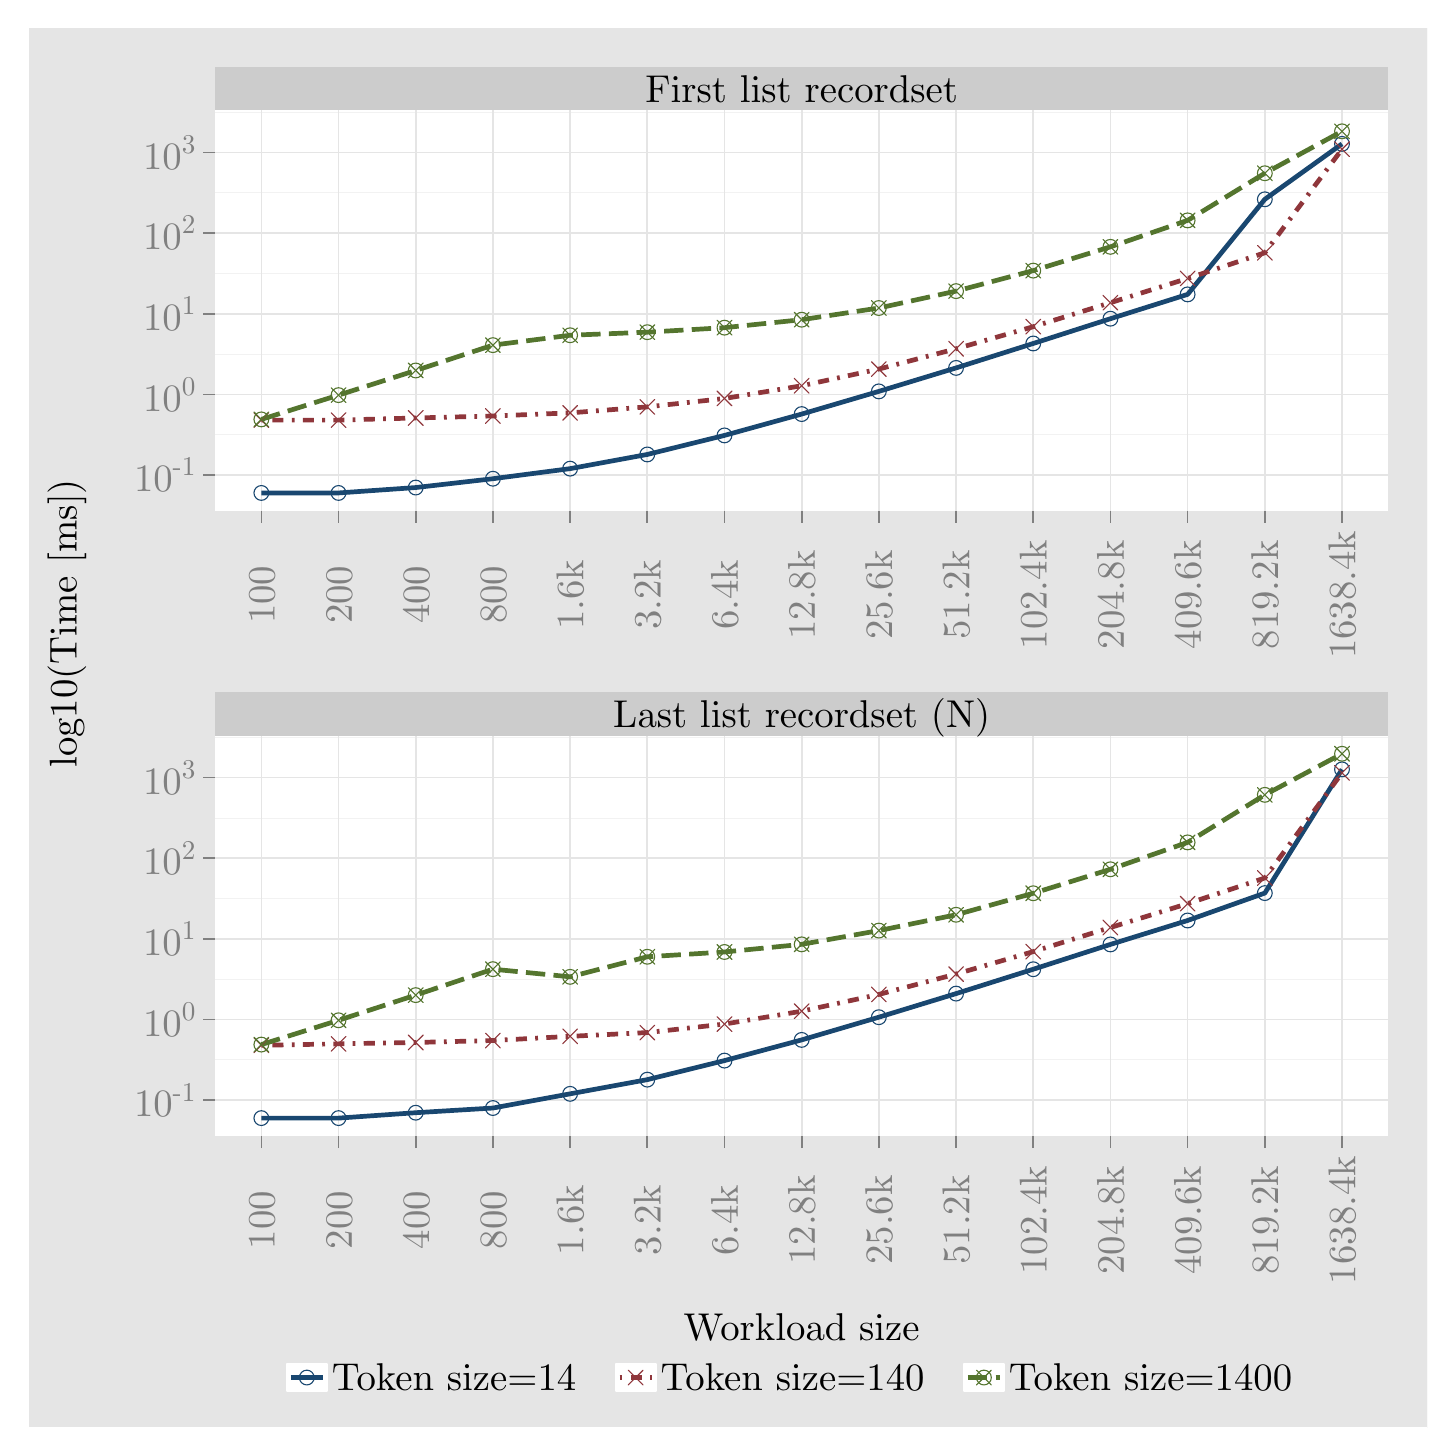
\begin{tikzpicture}[x=1pt,y=1pt]
\definecolor[named]{fillColor}{rgb}{1.00,1.00,1.00}
\path[use as bounding box,fill=fillColor,fill opacity=0.00] (0,0) rectangle (505.89,505.89);
\begin{scope}
\path[clip] (  0.00,  0.00) rectangle (505.89,505.89);
\definecolor[named]{drawColor}{rgb}{1.00,1.00,1.00}
\definecolor[named]{fillColor}{rgb}{0.90,0.90,0.90}

\path[draw=drawColor,line width= 0.6pt,line join=round,line cap=round,fill=fillColor] (  0.00, -0.00) rectangle (505.89,505.89);
\end{scope}
\begin{scope}
\path[clip] ( 67.70,331.18) rectangle (491.66,476.00);
\definecolor[named]{fillColor}{rgb}{1.00,1.00,1.00}

\path[fill=fillColor] ( 67.70,331.18) rectangle (491.66,476.00);
\definecolor[named]{drawColor}{rgb}{0.95,0.95,0.95}

\path[draw=drawColor,line width= 0.3pt,line join=round] ( 67.70,358.80) --
	(491.66,358.80);

\path[draw=drawColor,line width= 0.3pt,line join=round] ( 67.70,387.94) --
	(491.66,387.94);

\path[draw=drawColor,line width= 0.3pt,line join=round] ( 67.70,417.08) --
	(491.66,417.08);

\path[draw=drawColor,line width= 0.3pt,line join=round] ( 67.70,446.22) --
	(491.66,446.22);

\path[draw=drawColor,line width= 0.3pt,line join=round] ( 67.70,475.36) --
	(491.66,475.36);
\definecolor[named]{drawColor}{rgb}{0.90,0.90,0.90}

\path[draw=drawColor,line width= 0.6pt,line join=round] ( 67.70,344.23) --
	(491.66,344.23);

\path[draw=drawColor,line width= 0.6pt,line join=round] ( 67.70,373.37) --
	(491.66,373.37);

\path[draw=drawColor,line width= 0.6pt,line join=round] ( 67.70,402.51) --
	(491.66,402.51);

\path[draw=drawColor,line width= 0.6pt,line join=round] ( 67.70,431.65) --
	(491.66,431.65);

\path[draw=drawColor,line width= 0.6pt,line join=round] ( 67.70,460.79) --
	(491.66,460.79);

\path[draw=drawColor,line width= 0.6pt,line join=round] ( 84.44,331.18) --
	( 84.44,476.00);

\path[draw=drawColor,line width= 0.6pt,line join=round] (112.33,331.18) --
	(112.33,476.00);

\path[draw=drawColor,line width= 0.6pt,line join=round] (140.22,331.18) --
	(140.22,476.00);

\path[draw=drawColor,line width= 0.6pt,line join=round] (168.11,331.18) --
	(168.11,476.00);

\path[draw=drawColor,line width= 0.6pt,line join=round] (196.01,331.18) --
	(196.01,476.00);

\path[draw=drawColor,line width= 0.6pt,line join=round] (223.90,331.18) --
	(223.90,476.00);

\path[draw=drawColor,line width= 0.6pt,line join=round] (251.79,331.18) --
	(251.79,476.00);

\path[draw=drawColor,line width= 0.6pt,line join=round] (279.68,331.18) --
	(279.68,476.00);

\path[draw=drawColor,line width= 0.6pt,line join=round] (307.57,331.18) --
	(307.57,476.00);

\path[draw=drawColor,line width= 0.6pt,line join=round] (335.47,331.18) --
	(335.47,476.00);

\path[draw=drawColor,line width= 0.6pt,line join=round] (363.36,331.18) --
	(363.36,476.00);

\path[draw=drawColor,line width= 0.6pt,line join=round] (391.25,331.18) --
	(391.25,476.00);

\path[draw=drawColor,line width= 0.6pt,line join=round] (419.14,331.18) --
	(419.14,476.00);

\path[draw=drawColor,line width= 0.6pt,line join=round] (447.04,331.18) --
	(447.04,476.00);

\path[draw=drawColor,line width= 0.6pt,line join=round] (474.93,331.18) --
	(474.93,476.00);
\definecolor[named]{drawColor}{rgb}{0.10,0.28,0.44}

\path[draw=drawColor,line width= 1.7pt,line join=round] ( 84.44,337.76) --
	(112.33,337.76) --
	(140.22,339.71) --
	(168.11,342.90) --
	(196.01,346.54) --
	(223.90,351.67) --
	(251.79,358.55) --
	(279.68,366.26) --
	(307.57,374.46) --
	(335.47,382.94) --
	(363.36,391.77) --
	(391.25,400.72) --
	(419.14,409.51) --
	(447.04,443.87) --
	(474.93,463.89);
\definecolor[named]{drawColor}{rgb}{0.56,0.21,0.23}

\path[draw=drawColor,line width= 1.7pt,dash pattern=on 1pt off 3pt on 4pt off 3pt ,line join=round] ( 84.44,364.08) --
	(112.33,364.08) --
	(140.22,364.85) --
	(168.11,365.57) --
	(196.01,366.69) --
	(223.90,368.86) --
	(251.79,371.89) --
	(279.68,376.49) --
	(307.57,382.52) --
	(335.47,389.86) --
	(363.36,397.83) --
	(391.25,406.50) --
	(419.14,415.27) --
	(447.04,424.54) --
	(474.93,461.96);
\definecolor[named]{drawColor}{rgb}{0.33,0.46,0.18}

\path[draw=drawColor,line width= 1.7pt,dash pattern=on 7pt off 3pt ,line join=round] ( 84.44,364.34) --
	(112.33,373.11) --
	(140.22,382.01) --
	(168.11,391.17) --
	(196.01,394.74) --
	(223.90,395.85) --
	(251.79,397.48) --
	(279.68,400.36) --
	(307.57,404.58) --
	(335.47,410.69) --
	(363.36,418.10) --
	(391.25,426.69) --
	(419.14,436.25) --
	(447.04,453.28) --
	(474.93,468.43);
\definecolor[named]{drawColor}{rgb}{0.10,0.28,0.44}

\path[draw=drawColor,line width= 0.4pt,line join=round,line cap=round] ( 84.44,337.76) circle (  2.67);

\path[draw=drawColor,line width= 0.4pt,line join=round,line cap=round] (112.33,337.76) circle (  2.67);

\path[draw=drawColor,line width= 0.4pt,line join=round,line cap=round] (140.22,339.71) circle (  2.67);

\path[draw=drawColor,line width= 0.4pt,line join=round,line cap=round] (168.11,342.90) circle (  2.67);

\path[draw=drawColor,line width= 0.4pt,line join=round,line cap=round] (196.01,346.54) circle (  2.67);

\path[draw=drawColor,line width= 0.4pt,line join=round,line cap=round] (223.90,351.67) circle (  2.67);

\path[draw=drawColor,line width= 0.4pt,line join=round,line cap=round] (251.79,358.55) circle (  2.67);

\path[draw=drawColor,line width= 0.4pt,line join=round,line cap=round] (279.68,366.26) circle (  2.67);

\path[draw=drawColor,line width= 0.4pt,line join=round,line cap=round] (307.57,374.46) circle (  2.67);

\path[draw=drawColor,line width= 0.4pt,line join=round,line cap=round] (335.47,382.94) circle (  2.67);

\path[draw=drawColor,line width= 0.4pt,line join=round,line cap=round] (363.36,391.77) circle (  2.67);

\path[draw=drawColor,line width= 0.4pt,line join=round,line cap=round] (391.25,400.72) circle (  2.67);

\path[draw=drawColor,line width= 0.4pt,line join=round,line cap=round] (419.14,409.51) circle (  2.67);

\path[draw=drawColor,line width= 0.4pt,line join=round,line cap=round] (447.04,443.87) circle (  2.67);

\path[draw=drawColor,line width= 0.4pt,line join=round,line cap=round] (474.93,463.89) circle (  2.67);
\definecolor[named]{drawColor}{rgb}{0.56,0.21,0.23}

\path[draw=drawColor,line width= 0.4pt,line join=round,line cap=round,fill=fillColor] ( 81.77,361.41) -- ( 87.10,366.75);

\path[draw=drawColor,line width= 0.4pt,line join=round,line cap=round,fill=fillColor] ( 81.77,366.75) -- ( 87.10,361.41);

\path[draw=drawColor,line width= 0.4pt,line join=round,line cap=round,fill=fillColor] (109.66,361.41) -- (115.00,366.75);

\path[draw=drawColor,line width= 0.4pt,line join=round,line cap=round,fill=fillColor] (109.66,366.75) -- (115.00,361.41);

\path[draw=drawColor,line width= 0.4pt,line join=round,line cap=round,fill=fillColor] (137.55,362.18) -- (142.89,367.52);

\path[draw=drawColor,line width= 0.4pt,line join=round,line cap=round,fill=fillColor] (137.55,367.52) -- (142.89,362.18);

\path[draw=drawColor,line width= 0.4pt,line join=round,line cap=round,fill=fillColor] (165.45,362.90) -- (170.78,368.24);

\path[draw=drawColor,line width= 0.4pt,line join=round,line cap=round,fill=fillColor] (165.45,368.24) -- (170.78,362.90);

\path[draw=drawColor,line width= 0.4pt,line join=round,line cap=round,fill=fillColor] (193.34,364.02) -- (198.67,369.36);

\path[draw=drawColor,line width= 0.4pt,line join=round,line cap=round,fill=fillColor] (193.34,369.36) -- (198.67,364.02);

\path[draw=drawColor,line width= 0.4pt,line join=round,line cap=round,fill=fillColor] (221.23,366.19) -- (226.57,371.52);

\path[draw=drawColor,line width= 0.4pt,line join=round,line cap=round,fill=fillColor] (221.23,371.52) -- (226.57,366.19);

\path[draw=drawColor,line width= 0.4pt,line join=round,line cap=round,fill=fillColor] (249.12,369.23) -- (254.46,374.56);

\path[draw=drawColor,line width= 0.4pt,line join=round,line cap=round,fill=fillColor] (249.12,374.56) -- (254.46,369.23);

\path[draw=drawColor,line width= 0.4pt,line join=round,line cap=round,fill=fillColor] (277.01,373.83) -- (282.35,379.16);

\path[draw=drawColor,line width= 0.4pt,line join=round,line cap=round,fill=fillColor] (277.01,379.16) -- (282.35,373.83);

\path[draw=drawColor,line width= 0.4pt,line join=round,line cap=round,fill=fillColor] (304.91,379.85) -- (310.24,385.18);

\path[draw=drawColor,line width= 0.4pt,line join=round,line cap=round,fill=fillColor] (304.91,385.18) -- (310.24,379.85);

\path[draw=drawColor,line width= 0.4pt,line join=round,line cap=round,fill=fillColor] (332.80,387.19) -- (338.13,392.53);

\path[draw=drawColor,line width= 0.4pt,line join=round,line cap=round,fill=fillColor] (332.80,392.53) -- (338.13,387.19);

\path[draw=drawColor,line width= 0.4pt,line join=round,line cap=round,fill=fillColor] (360.69,395.17) -- (366.03,400.50);

\path[draw=drawColor,line width= 0.4pt,line join=round,line cap=round,fill=fillColor] (360.69,400.50) -- (366.03,395.17);

\path[draw=drawColor,line width= 0.4pt,line join=round,line cap=round,fill=fillColor] (388.58,403.83) -- (393.92,409.16);

\path[draw=drawColor,line width= 0.4pt,line join=round,line cap=round,fill=fillColor] (388.58,409.16) -- (393.92,403.83);

\path[draw=drawColor,line width= 0.4pt,line join=round,line cap=round,fill=fillColor] (416.48,412.60) -- (421.81,417.93);

\path[draw=drawColor,line width= 0.4pt,line join=round,line cap=round,fill=fillColor] (416.48,417.93) -- (421.81,412.60);

\path[draw=drawColor,line width= 0.4pt,line join=round,line cap=round,fill=fillColor] (444.37,421.88) -- (449.70,427.21);

\path[draw=drawColor,line width= 0.4pt,line join=round,line cap=round,fill=fillColor] (444.37,427.21) -- (449.70,421.88);

\path[draw=drawColor,line width= 0.4pt,line join=round,line cap=round,fill=fillColor] (472.26,459.30) -- (477.60,464.63);

\path[draw=drawColor,line width= 0.4pt,line join=round,line cap=round,fill=fillColor] (472.26,464.63) -- (477.60,459.30);
\definecolor[named]{drawColor}{rgb}{0.33,0.46,0.18}

\path[draw=drawColor,line width= 0.4pt,line join=round,line cap=round] ( 84.44,364.34) circle (  2.67);

\path[draw=drawColor,line width= 0.4pt,line join=round,line cap=round] ( 81.77,361.67) -- ( 87.10,367.01);

\path[draw=drawColor,line width= 0.4pt,line join=round,line cap=round] ( 81.77,367.01) -- ( 87.10,361.67);

\path[draw=drawColor,line width= 0.4pt,line join=round,line cap=round] (112.33,373.11) circle (  2.67);

\path[draw=drawColor,line width= 0.4pt,line join=round,line cap=round] (109.66,370.45) -- (115.00,375.78);

\path[draw=drawColor,line width= 0.4pt,line join=round,line cap=round] (109.66,375.78) -- (115.00,370.45);

\path[draw=drawColor,line width= 0.4pt,line join=round,line cap=round] (140.22,382.01) circle (  2.67);

\path[draw=drawColor,line width= 0.4pt,line join=round,line cap=round] (137.55,379.35) -- (142.89,384.68);

\path[draw=drawColor,line width= 0.4pt,line join=round,line cap=round] (137.55,384.68) -- (142.89,379.35);

\path[draw=drawColor,line width= 0.4pt,line join=round,line cap=round] (168.11,391.17) circle (  2.67);

\path[draw=drawColor,line width= 0.4pt,line join=round,line cap=round] (165.45,388.50) -- (170.78,393.83);

\path[draw=drawColor,line width= 0.4pt,line join=round,line cap=round] (165.45,393.83) -- (170.78,388.50);

\path[draw=drawColor,line width= 0.4pt,line join=round,line cap=round] (196.01,394.74) circle (  2.67);

\path[draw=drawColor,line width= 0.4pt,line join=round,line cap=round] (193.34,392.07) -- (198.67,397.40);

\path[draw=drawColor,line width= 0.4pt,line join=round,line cap=round] (193.34,397.40) -- (198.67,392.07);

\path[draw=drawColor,line width= 0.4pt,line join=round,line cap=round] (223.90,395.85) circle (  2.67);

\path[draw=drawColor,line width= 0.4pt,line join=round,line cap=round] (221.23,393.19) -- (226.57,398.52);

\path[draw=drawColor,line width= 0.4pt,line join=round,line cap=round] (221.23,398.52) -- (226.57,393.19);

\path[draw=drawColor,line width= 0.4pt,line join=round,line cap=round] (251.79,397.48) circle (  2.67);

\path[draw=drawColor,line width= 0.4pt,line join=round,line cap=round] (249.12,394.81) -- (254.46,400.15);

\path[draw=drawColor,line width= 0.4pt,line join=round,line cap=round] (249.12,400.15) -- (254.46,394.81);

\path[draw=drawColor,line width= 0.4pt,line join=round,line cap=round] (279.68,400.36) circle (  2.67);

\path[draw=drawColor,line width= 0.4pt,line join=round,line cap=round] (277.01,397.70) -- (282.35,403.03);

\path[draw=drawColor,line width= 0.4pt,line join=round,line cap=round] (277.01,403.03) -- (282.35,397.70);

\path[draw=drawColor,line width= 0.4pt,line join=round,line cap=round] (307.57,404.58) circle (  2.67);

\path[draw=drawColor,line width= 0.4pt,line join=round,line cap=round] (304.91,401.92) -- (310.24,407.25);

\path[draw=drawColor,line width= 0.4pt,line join=round,line cap=round] (304.91,407.25) -- (310.24,401.92);

\path[draw=drawColor,line width= 0.4pt,line join=round,line cap=round] (335.47,410.69) circle (  2.67);

\path[draw=drawColor,line width= 0.4pt,line join=round,line cap=round] (332.80,408.03) -- (338.13,413.36);

\path[draw=drawColor,line width= 0.4pt,line join=round,line cap=round] (332.80,413.36) -- (338.13,408.03);

\path[draw=drawColor,line width= 0.4pt,line join=round,line cap=round] (363.36,418.10) circle (  2.67);

\path[draw=drawColor,line width= 0.4pt,line join=round,line cap=round] (360.69,415.43) -- (366.03,420.76);

\path[draw=drawColor,line width= 0.4pt,line join=round,line cap=round] (360.69,420.76) -- (366.03,415.43);

\path[draw=drawColor,line width= 0.4pt,line join=round,line cap=round] (391.25,426.69) circle (  2.67);

\path[draw=drawColor,line width= 0.4pt,line join=round,line cap=round] (388.58,424.03) -- (393.92,429.36);

\path[draw=drawColor,line width= 0.4pt,line join=round,line cap=round] (388.58,429.36) -- (393.92,424.03);

\path[draw=drawColor,line width= 0.4pt,line join=round,line cap=round] (419.14,436.25) circle (  2.67);

\path[draw=drawColor,line width= 0.4pt,line join=round,line cap=round] (416.48,433.59) -- (421.81,438.92);

\path[draw=drawColor,line width= 0.4pt,line join=round,line cap=round] (416.48,438.92) -- (421.81,433.59);

\path[draw=drawColor,line width= 0.4pt,line join=round,line cap=round] (447.04,453.28) circle (  2.67);

\path[draw=drawColor,line width= 0.4pt,line join=round,line cap=round] (444.37,450.61) -- (449.70,455.95);

\path[draw=drawColor,line width= 0.4pt,line join=round,line cap=round] (444.37,455.95) -- (449.70,450.61);

\path[draw=drawColor,line width= 0.4pt,line join=round,line cap=round] (474.93,468.43) circle (  2.67);

\path[draw=drawColor,line width= 0.4pt,line join=round,line cap=round] (472.26,465.76) -- (477.60,471.09);

\path[draw=drawColor,line width= 0.4pt,line join=round,line cap=round] (472.26,471.09) -- (477.60,465.76);
\end{scope}
\begin{scope}
\path[clip] ( 67.70,105.27) rectangle (491.66,250.09);
\definecolor[named]{fillColor}{rgb}{1.00,1.00,1.00}

\path[fill=fillColor] ( 67.70,105.27) rectangle (491.66,250.09);
\definecolor[named]{drawColor}{rgb}{0.95,0.95,0.95}

\path[draw=drawColor,line width= 0.3pt,line join=round] ( 67.70,132.89) --
	(491.66,132.89);

\path[draw=drawColor,line width= 0.3pt,line join=round] ( 67.70,162.03) --
	(491.66,162.03);

\path[draw=drawColor,line width= 0.3pt,line join=round] ( 67.70,191.17) --
	(491.66,191.17);

\path[draw=drawColor,line width= 0.3pt,line join=round] ( 67.70,220.32) --
	(491.66,220.32);

\path[draw=drawColor,line width= 0.3pt,line join=round] ( 67.70,249.46) --
	(491.66,249.46);
\definecolor[named]{drawColor}{rgb}{0.90,0.90,0.90}

\path[draw=drawColor,line width= 0.6pt,line join=round] ( 67.70,118.32) --
	(491.66,118.32);

\path[draw=drawColor,line width= 0.6pt,line join=round] ( 67.70,147.46) --
	(491.66,147.46);

\path[draw=drawColor,line width= 0.6pt,line join=round] ( 67.70,176.60) --
	(491.66,176.60);

\path[draw=drawColor,line width= 0.6pt,line join=round] ( 67.70,205.75) --
	(491.66,205.75);

\path[draw=drawColor,line width= 0.6pt,line join=round] ( 67.70,234.89) --
	(491.66,234.89);

\path[draw=drawColor,line width= 0.6pt,line join=round] ( 84.44,105.27) --
	( 84.44,250.09);

\path[draw=drawColor,line width= 0.6pt,line join=round] (112.33,105.27) --
	(112.33,250.09);

\path[draw=drawColor,line width= 0.6pt,line join=round] (140.22,105.27) --
	(140.22,250.09);

\path[draw=drawColor,line width= 0.6pt,line join=round] (168.11,105.27) --
	(168.11,250.09);

\path[draw=drawColor,line width= 0.6pt,line join=round] (196.01,105.27) --
	(196.01,250.09);

\path[draw=drawColor,line width= 0.6pt,line join=round] (223.90,105.27) --
	(223.90,250.09);

\path[draw=drawColor,line width= 0.6pt,line join=round] (251.79,105.27) --
	(251.79,250.09);

\path[draw=drawColor,line width= 0.6pt,line join=round] (279.68,105.27) --
	(279.68,250.09);

\path[draw=drawColor,line width= 0.6pt,line join=round] (307.57,105.27) --
	(307.57,250.09);

\path[draw=drawColor,line width= 0.6pt,line join=round] (335.47,105.27) --
	(335.47,250.09);

\path[draw=drawColor,line width= 0.6pt,line join=round] (363.36,105.27) --
	(363.36,250.09);

\path[draw=drawColor,line width= 0.6pt,line join=round] (391.25,105.27) --
	(391.25,250.09);

\path[draw=drawColor,line width= 0.6pt,line join=round] (419.14,105.27) --
	(419.14,250.09);

\path[draw=drawColor,line width= 0.6pt,line join=round] (447.04,105.27) --
	(447.04,250.09);

\path[draw=drawColor,line width= 0.6pt,line join=round] (474.93,105.27) --
	(474.93,250.09);
\definecolor[named]{drawColor}{rgb}{0.10,0.28,0.44}

\path[draw=drawColor,line width= 1.7pt,line join=round] ( 84.44,111.86) --
	(112.33,111.86) --
	(140.22,113.81) --
	(168.11,115.50) --
	(196.01,120.63) --
	(223.90,125.76) --
	(251.79,132.64) --
	(279.68,140.12) --
	(307.57,148.32) --
	(335.47,156.85) --
	(363.36,165.65) --
	(391.25,174.62) --
	(419.14,183.27) --
	(447.04,193.17) --
	(474.93,237.88);
\definecolor[named]{drawColor}{rgb}{0.56,0.21,0.23}

\path[draw=drawColor,line width= 1.7pt,dash pattern=on 1pt off 3pt on 4pt off 3pt ,line join=round] ( 84.44,138.17) --
	(112.33,138.69) --
	(140.22,139.19) --
	(168.11,139.90) --
	(196.01,141.41) --
	(223.90,142.77) --
	(251.79,145.84) --
	(279.68,150.49) --
	(307.57,156.55) --
	(335.47,163.92) --
	(363.36,172.02) --
	(391.25,180.73) --
	(419.14,189.35) --
	(447.04,198.63) --
	(474.93,236.61);
\definecolor[named]{drawColor}{rgb}{0.33,0.46,0.18}

\path[draw=drawColor,line width= 1.7pt,dash pattern=on 7pt off 3pt ,line join=round] ( 84.44,138.43) --
	(112.33,147.21) --
	(140.22,156.30) --
	(168.11,165.68) --
	(196.01,162.91) --
	(223.90,170.16) --
	(251.79,171.89) --
	(279.68,174.65) --
	(307.57,179.62) --
	(335.47,185.33) --
	(363.36,193.11) --
	(391.25,201.77) --
	(419.14,211.49) --
	(447.04,228.67) --
	(474.93,243.51);
\definecolor[named]{drawColor}{rgb}{0.10,0.28,0.44}

\path[draw=drawColor,line width= 0.4pt,line join=round,line cap=round] ( 84.44,111.86) circle (  2.67);

\path[draw=drawColor,line width= 0.4pt,line join=round,line cap=round] (112.33,111.86) circle (  2.67);

\path[draw=drawColor,line width= 0.4pt,line join=round,line cap=round] (140.22,113.81) circle (  2.67);

\path[draw=drawColor,line width= 0.4pt,line join=round,line cap=round] (168.11,115.50) circle (  2.67);

\path[draw=drawColor,line width= 0.4pt,line join=round,line cap=round] (196.01,120.63) circle (  2.67);

\path[draw=drawColor,line width= 0.4pt,line join=round,line cap=round] (223.90,125.76) circle (  2.67);

\path[draw=drawColor,line width= 0.4pt,line join=round,line cap=round] (251.79,132.64) circle (  2.67);

\path[draw=drawColor,line width= 0.4pt,line join=round,line cap=round] (279.68,140.12) circle (  2.67);

\path[draw=drawColor,line width= 0.4pt,line join=round,line cap=round] (307.57,148.32) circle (  2.67);

\path[draw=drawColor,line width= 0.4pt,line join=round,line cap=round] (335.47,156.85) circle (  2.67);

\path[draw=drawColor,line width= 0.4pt,line join=round,line cap=round] (363.36,165.65) circle (  2.67);

\path[draw=drawColor,line width= 0.4pt,line join=round,line cap=round] (391.25,174.62) circle (  2.67);

\path[draw=drawColor,line width= 0.4pt,line join=round,line cap=round] (419.14,183.27) circle (  2.67);

\path[draw=drawColor,line width= 0.4pt,line join=round,line cap=round] (447.04,193.17) circle (  2.67);

\path[draw=drawColor,line width= 0.4pt,line join=round,line cap=round] (474.93,237.88) circle (  2.67);
\definecolor[named]{drawColor}{rgb}{0.56,0.21,0.23}

\path[draw=drawColor,line width= 0.4pt,line join=round,line cap=round,fill=fillColor] ( 81.77,135.51) -- ( 87.10,140.84);

\path[draw=drawColor,line width= 0.4pt,line join=round,line cap=round,fill=fillColor] ( 81.77,140.84) -- ( 87.10,135.51);

\path[draw=drawColor,line width= 0.4pt,line join=round,line cap=round,fill=fillColor] (109.66,136.02) -- (115.00,141.36);

\path[draw=drawColor,line width= 0.4pt,line join=round,line cap=round,fill=fillColor] (109.66,141.36) -- (115.00,136.02);

\path[draw=drawColor,line width= 0.4pt,line join=round,line cap=round,fill=fillColor] (137.55,136.52) -- (142.89,141.85);

\path[draw=drawColor,line width= 0.4pt,line join=round,line cap=round,fill=fillColor] (137.55,141.85) -- (142.89,136.52);

\path[draw=drawColor,line width= 0.4pt,line join=round,line cap=round,fill=fillColor] (165.45,137.23) -- (170.78,142.56);

\path[draw=drawColor,line width= 0.4pt,line join=round,line cap=round,fill=fillColor] (165.45,142.56) -- (170.78,137.23);

\path[draw=drawColor,line width= 0.4pt,line join=round,line cap=round,fill=fillColor] (193.34,138.75) -- (198.67,144.08);

\path[draw=drawColor,line width= 0.4pt,line join=round,line cap=round,fill=fillColor] (193.34,144.08) -- (198.67,138.75);

\path[draw=drawColor,line width= 0.4pt,line join=round,line cap=round,fill=fillColor] (221.23,140.10) -- (226.57,145.43);

\path[draw=drawColor,line width= 0.4pt,line join=round,line cap=round,fill=fillColor] (221.23,145.43) -- (226.57,140.10);

\path[draw=drawColor,line width= 0.4pt,line join=round,line cap=round,fill=fillColor] (249.12,143.18) -- (254.46,148.51);

\path[draw=drawColor,line width= 0.4pt,line join=round,line cap=round,fill=fillColor] (249.12,148.51) -- (254.46,143.18);

\path[draw=drawColor,line width= 0.4pt,line join=round,line cap=round,fill=fillColor] (277.01,147.82) -- (282.35,153.16);

\path[draw=drawColor,line width= 0.4pt,line join=round,line cap=round,fill=fillColor] (277.01,153.16) -- (282.35,147.82);

\path[draw=drawColor,line width= 0.4pt,line join=round,line cap=round,fill=fillColor] (304.91,153.88) -- (310.24,159.21);

\path[draw=drawColor,line width= 0.4pt,line join=round,line cap=round,fill=fillColor] (304.91,159.21) -- (310.24,153.88);

\path[draw=drawColor,line width= 0.4pt,line join=round,line cap=round,fill=fillColor] (332.80,161.25) -- (338.13,166.59);

\path[draw=drawColor,line width= 0.4pt,line join=round,line cap=round,fill=fillColor] (332.80,166.59) -- (338.13,161.25);

\path[draw=drawColor,line width= 0.4pt,line join=round,line cap=round,fill=fillColor] (360.69,169.35) -- (366.03,174.68);

\path[draw=drawColor,line width= 0.4pt,line join=round,line cap=round,fill=fillColor] (360.69,174.68) -- (366.03,169.35);

\path[draw=drawColor,line width= 0.4pt,line join=round,line cap=round,fill=fillColor] (388.58,178.07) -- (393.92,183.40);

\path[draw=drawColor,line width= 0.4pt,line join=round,line cap=round,fill=fillColor] (388.58,183.40) -- (393.92,178.07);

\path[draw=drawColor,line width= 0.4pt,line join=round,line cap=round,fill=fillColor] (416.48,186.68) -- (421.81,192.02);

\path[draw=drawColor,line width= 0.4pt,line join=round,line cap=round,fill=fillColor] (416.48,192.02) -- (421.81,186.68);

\path[draw=drawColor,line width= 0.4pt,line join=round,line cap=round,fill=fillColor] (444.37,195.96) -- (449.70,201.30);

\path[draw=drawColor,line width= 0.4pt,line join=round,line cap=round,fill=fillColor] (444.37,201.30) -- (449.70,195.96);

\path[draw=drawColor,line width= 0.4pt,line join=round,line cap=round,fill=fillColor] (472.26,233.94) -- (477.60,239.27);

\path[draw=drawColor,line width= 0.4pt,line join=round,line cap=round,fill=fillColor] (472.26,239.27) -- (477.60,233.94);
\definecolor[named]{drawColor}{rgb}{0.33,0.46,0.18}

\path[draw=drawColor,line width= 0.4pt,line join=round,line cap=round] ( 84.44,138.43) circle (  2.67);

\path[draw=drawColor,line width= 0.4pt,line join=round,line cap=round] ( 81.77,135.77) -- ( 87.10,141.10);

\path[draw=drawColor,line width= 0.4pt,line join=round,line cap=round] ( 81.77,141.10) -- ( 87.10,135.77);

\path[draw=drawColor,line width= 0.4pt,line join=round,line cap=round] (112.33,147.21) circle (  2.67);

\path[draw=drawColor,line width= 0.4pt,line join=round,line cap=round] (109.66,144.54) -- (115.00,149.87);

\path[draw=drawColor,line width= 0.4pt,line join=round,line cap=round] (109.66,149.87) -- (115.00,144.54);

\path[draw=drawColor,line width= 0.4pt,line join=round,line cap=round] (140.22,156.30) circle (  2.67);

\path[draw=drawColor,line width= 0.4pt,line join=round,line cap=round] (137.55,153.63) -- (142.89,158.97);

\path[draw=drawColor,line width= 0.4pt,line join=round,line cap=round] (137.55,158.97) -- (142.89,153.63);

\path[draw=drawColor,line width= 0.4pt,line join=round,line cap=round] (168.11,165.68) circle (  2.67);

\path[draw=drawColor,line width= 0.4pt,line join=round,line cap=round] (165.45,163.02) -- (170.78,168.35);

\path[draw=drawColor,line width= 0.4pt,line join=round,line cap=round] (165.45,168.35) -- (170.78,163.02);

\path[draw=drawColor,line width= 0.4pt,line join=round,line cap=round] (196.01,162.91) circle (  2.67);

\path[draw=drawColor,line width= 0.4pt,line join=round,line cap=round] (193.34,160.25) -- (198.67,165.58);

\path[draw=drawColor,line width= 0.4pt,line join=round,line cap=round] (193.34,165.58) -- (198.67,160.25);

\path[draw=drawColor,line width= 0.4pt,line join=round,line cap=round] (223.90,170.16) circle (  2.67);

\path[draw=drawColor,line width= 0.4pt,line join=round,line cap=round] (221.23,167.49) -- (226.57,172.83);

\path[draw=drawColor,line width= 0.4pt,line join=round,line cap=round] (221.23,172.83) -- (226.57,167.49);

\path[draw=drawColor,line width= 0.4pt,line join=round,line cap=round] (251.79,171.89) circle (  2.67);

\path[draw=drawColor,line width= 0.4pt,line join=round,line cap=round] (249.12,169.22) -- (254.46,174.56);

\path[draw=drawColor,line width= 0.4pt,line join=round,line cap=round] (249.12,174.56) -- (254.46,169.22);

\path[draw=drawColor,line width= 0.4pt,line join=round,line cap=round] (279.68,174.65) circle (  2.67);

\path[draw=drawColor,line width= 0.4pt,line join=round,line cap=round] (277.01,171.98) -- (282.35,177.32);

\path[draw=drawColor,line width= 0.4pt,line join=round,line cap=round] (277.01,177.32) -- (282.35,171.98);

\path[draw=drawColor,line width= 0.4pt,line join=round,line cap=round] (307.57,179.62) circle (  2.67);

\path[draw=drawColor,line width= 0.4pt,line join=round,line cap=round] (304.91,176.95) -- (310.24,182.29);

\path[draw=drawColor,line width= 0.4pt,line join=round,line cap=round] (304.91,182.29) -- (310.24,176.95);

\path[draw=drawColor,line width= 0.4pt,line join=round,line cap=round] (335.47,185.33) circle (  2.67);

\path[draw=drawColor,line width= 0.4pt,line join=round,line cap=round] (332.80,182.66) -- (338.13,187.99);

\path[draw=drawColor,line width= 0.4pt,line join=round,line cap=round] (332.80,187.99) -- (338.13,182.66);

\path[draw=drawColor,line width= 0.4pt,line join=round,line cap=round] (363.36,193.11) circle (  2.67);

\path[draw=drawColor,line width= 0.4pt,line join=round,line cap=round] (360.69,190.44) -- (366.03,195.78);

\path[draw=drawColor,line width= 0.4pt,line join=round,line cap=round] (360.69,195.78) -- (366.03,190.44);

\path[draw=drawColor,line width= 0.4pt,line join=round,line cap=round] (391.25,201.77) circle (  2.67);

\path[draw=drawColor,line width= 0.4pt,line join=round,line cap=round] (388.58,199.10) -- (393.92,204.43);

\path[draw=drawColor,line width= 0.4pt,line join=round,line cap=round] (388.58,204.43) -- (393.92,199.10);

\path[draw=drawColor,line width= 0.4pt,line join=round,line cap=round] (419.14,211.49) circle (  2.67);

\path[draw=drawColor,line width= 0.4pt,line join=round,line cap=round] (416.48,208.82) -- (421.81,214.16);

\path[draw=drawColor,line width= 0.4pt,line join=round,line cap=round] (416.48,214.16) -- (421.81,208.82);

\path[draw=drawColor,line width= 0.4pt,line join=round,line cap=round] (447.04,228.67) circle (  2.67);

\path[draw=drawColor,line width= 0.4pt,line join=round,line cap=round] (444.37,226.00) -- (449.70,231.33);

\path[draw=drawColor,line width= 0.4pt,line join=round,line cap=round] (444.37,231.33) -- (449.70,226.00);

\path[draw=drawColor,line width= 0.4pt,line join=round,line cap=round] (474.93,243.51) circle (  2.67);

\path[draw=drawColor,line width= 0.4pt,line join=round,line cap=round] (472.26,240.84) -- (477.60,246.18);

\path[draw=drawColor,line width= 0.4pt,line join=round,line cap=round] (472.26,246.18) -- (477.60,240.84);
\end{scope}
\begin{scope}
\path[clip] (  0.00,  0.00) rectangle (505.89,505.89);
\definecolor[named]{fillColor}{rgb}{0.80,0.80,0.80}

\path[fill=fillColor] ( 67.70,476.00) rectangle (491.66,491.66);
\definecolor[named]{drawColor}{rgb}{0.00,0.00,0.00}

\node[text=drawColor,anchor=base,inner sep=0pt, outer sep=0pt, scale=  1.40] at (279.68,479.01) {First list recordset };
\end{scope}
\begin{scope}
\path[clip] (  0.00,  0.00) rectangle (505.89,505.89);
\definecolor[named]{fillColor}{rgb}{0.80,0.80,0.80}

\path[fill=fillColor] ( 67.70,250.09) rectangle (491.66,265.76);
\definecolor[named]{drawColor}{rgb}{0.00,0.00,0.00}

\node[text=drawColor,anchor=base,inner sep=0pt, outer sep=0pt, scale=  1.40] at (279.68,253.10) {Last list recordset (N) };
\end{scope}
\begin{scope}
\path[clip] (  0.00,  0.00) rectangle (505.89,505.89);
\definecolor[named]{drawColor}{rgb}{0.50,0.50,0.50}

\node[text=drawColor,anchor=base west,inner sep=0pt, outer sep=0pt, scale=  1.40] at ( 38.43,338.22) {10};

\node[text=drawColor,anchor=base west,inner sep=0pt, outer sep=0pt, scale=  0.98] at ( 52.42,343.95) {-};

\node[text=drawColor,anchor=base west,inner sep=0pt, outer sep=0pt, scale=  0.98] at ( 55.69,343.95) {1};

\node[text=drawColor,anchor=base west,inner sep=0pt, outer sep=0pt, scale=  1.40] at ( 41.69,367.36) {10};

\node[text=drawColor,anchor=base west,inner sep=0pt, outer sep=0pt, scale=  0.98] at ( 55.69,373.09) {0};

\node[text=drawColor,anchor=base west,inner sep=0pt, outer sep=0pt, scale=  1.40] at ( 41.69,396.51) {10};

\node[text=drawColor,anchor=base west,inner sep=0pt, outer sep=0pt, scale=  0.98] at ( 55.69,402.23) {1};

\node[text=drawColor,anchor=base west,inner sep=0pt, outer sep=0pt, scale=  1.40] at ( 41.69,425.65) {10};

\node[text=drawColor,anchor=base west,inner sep=0pt, outer sep=0pt, scale=  0.98] at ( 55.69,431.37) {2};

\node[text=drawColor,anchor=base west,inner sep=0pt, outer sep=0pt, scale=  1.40] at ( 41.69,454.79) {10};

\node[text=drawColor,anchor=base west,inner sep=0pt, outer sep=0pt, scale=  0.98] at ( 55.69,460.51) {3};
\end{scope}
\begin{scope}
\path[clip] (  0.00,  0.00) rectangle (505.89,505.89);
\definecolor[named]{drawColor}{rgb}{0.50,0.50,0.50}

\path[draw=drawColor,line width= 0.6pt,line join=round] ( 63.43,344.23) --
	( 67.70,344.23);

\path[draw=drawColor,line width= 0.6pt,line join=round] ( 63.43,373.37) --
	( 67.70,373.37);

\path[draw=drawColor,line width= 0.6pt,line join=round] ( 63.43,402.51) --
	( 67.70,402.51);

\path[draw=drawColor,line width= 0.6pt,line join=round] ( 63.43,431.65) --
	( 67.70,431.65);

\path[draw=drawColor,line width= 0.6pt,line join=round] ( 63.43,460.79) --
	( 67.70,460.79);
\end{scope}
\begin{scope}
\path[clip] (  0.00,  0.00) rectangle (505.89,505.89);
\definecolor[named]{drawColor}{rgb}{0.50,0.50,0.50}

\node[text=drawColor,anchor=base west,inner sep=0pt, outer sep=0pt, scale=  1.40] at ( 38.43,112.32) {10};

\node[text=drawColor,anchor=base west,inner sep=0pt, outer sep=0pt, scale=  0.98] at ( 52.42,118.04) {-};

\node[text=drawColor,anchor=base west,inner sep=0pt, outer sep=0pt, scale=  0.98] at ( 55.69,118.04) {1};

\node[text=drawColor,anchor=base west,inner sep=0pt, outer sep=0pt, scale=  1.40] at ( 41.69,141.46) {10};

\node[text=drawColor,anchor=base west,inner sep=0pt, outer sep=0pt, scale=  0.98] at ( 55.69,147.18) {0};

\node[text=drawColor,anchor=base west,inner sep=0pt, outer sep=0pt, scale=  1.40] at ( 41.69,170.60) {10};

\node[text=drawColor,anchor=base west,inner sep=0pt, outer sep=0pt, scale=  0.98] at ( 55.69,176.32) {1};

\node[text=drawColor,anchor=base west,inner sep=0pt, outer sep=0pt, scale=  1.40] at ( 41.69,199.74) {10};

\node[text=drawColor,anchor=base west,inner sep=0pt, outer sep=0pt, scale=  0.98] at ( 55.69,205.46) {2};

\node[text=drawColor,anchor=base west,inner sep=0pt, outer sep=0pt, scale=  1.40] at ( 41.69,228.88) {10};

\node[text=drawColor,anchor=base west,inner sep=0pt, outer sep=0pt, scale=  0.98] at ( 55.69,234.61) {3};
\end{scope}
\begin{scope}
\path[clip] (  0.00,  0.00) rectangle (505.89,505.89);
\definecolor[named]{drawColor}{rgb}{0.50,0.50,0.50}

\path[draw=drawColor,line width= 0.6pt,line join=round] ( 63.43,118.32) --
	( 67.70,118.32);

\path[draw=drawColor,line width= 0.6pt,line join=round] ( 63.43,147.46) --
	( 67.70,147.46);

\path[draw=drawColor,line width= 0.6pt,line join=round] ( 63.43,176.60) --
	( 67.70,176.60);

\path[draw=drawColor,line width= 0.6pt,line join=round] ( 63.43,205.75) --
	( 67.70,205.75);

\path[draw=drawColor,line width= 0.6pt,line join=round] ( 63.43,234.89) --
	( 67.70,234.89);
\end{scope}
\begin{scope}
\path[clip] (  0.00,  0.00) rectangle (505.89,505.89);
\definecolor[named]{drawColor}{rgb}{0.50,0.50,0.50}

\path[draw=drawColor,line width= 0.6pt,line join=round] ( 84.44,326.91) --
	( 84.44,331.18);

\path[draw=drawColor,line width= 0.6pt,line join=round] (112.33,326.91) --
	(112.33,331.18);

\path[draw=drawColor,line width= 0.6pt,line join=round] (140.22,326.91) --
	(140.22,331.18);

\path[draw=drawColor,line width= 0.6pt,line join=round] (168.11,326.91) --
	(168.11,331.18);

\path[draw=drawColor,line width= 0.6pt,line join=round] (196.01,326.91) --
	(196.01,331.18);

\path[draw=drawColor,line width= 0.6pt,line join=round] (223.90,326.91) --
	(223.90,331.18);

\path[draw=drawColor,line width= 0.6pt,line join=round] (251.79,326.91) --
	(251.79,331.18);

\path[draw=drawColor,line width= 0.6pt,line join=round] (279.68,326.91) --
	(279.68,331.18);

\path[draw=drawColor,line width= 0.6pt,line join=round] (307.57,326.91) --
	(307.57,331.18);

\path[draw=drawColor,line width= 0.6pt,line join=round] (335.47,326.91) --
	(335.47,331.18);

\path[draw=drawColor,line width= 0.6pt,line join=round] (363.36,326.91) --
	(363.36,331.18);

\path[draw=drawColor,line width= 0.6pt,line join=round] (391.25,326.91) --
	(391.25,331.18);

\path[draw=drawColor,line width= 0.6pt,line join=round] (419.14,326.91) --
	(419.14,331.18);

\path[draw=drawColor,line width= 0.6pt,line join=round] (447.04,326.91) --
	(447.04,331.18);

\path[draw=drawColor,line width= 0.6pt,line join=round] (474.93,326.91) --
	(474.93,331.18);
\end{scope}
\begin{scope}
\path[clip] (  0.00,  0.00) rectangle (505.89,505.89);
\definecolor[named]{drawColor}{rgb}{0.50,0.50,0.50}

\node[text=drawColor,rotate= 90.00,anchor=base,inner sep=0pt, outer sep=0pt, scale=  1.40] at ( 89.26,300.93) {100};

\node[text=drawColor,rotate= 90.00,anchor=base,inner sep=0pt, outer sep=0pt, scale=  1.40] at (117.15,300.93) {200};

\node[text=drawColor,rotate= 90.00,anchor=base,inner sep=0pt, outer sep=0pt, scale=  1.40] at (145.04,300.93) {400};

\node[text=drawColor,rotate= 90.00,anchor=base,inner sep=0pt, outer sep=0pt, scale=  1.40] at (172.93,300.93) {800};

\node[text=drawColor,rotate= 90.00,anchor=base,inner sep=0pt, outer sep=0pt, scale=  1.40] at (200.83,300.93) {1.6k};

\node[text=drawColor,rotate= 90.00,anchor=base,inner sep=0pt, outer sep=0pt, scale=  1.40] at (228.72,300.93) {3.2k};

\node[text=drawColor,rotate= 90.00,anchor=base,inner sep=0pt, outer sep=0pt, scale=  1.40] at (256.61,300.93) {6.4k};

\node[text=drawColor,rotate= 90.00,anchor=base,inner sep=0pt, outer sep=0pt, scale=  1.40] at (284.50,300.93) {12.8k};

\node[text=drawColor,rotate= 90.00,anchor=base,inner sep=0pt, outer sep=0pt, scale=  1.40] at (312.40,300.93) {25.6k};

\node[text=drawColor,rotate= 90.00,anchor=base,inner sep=0pt, outer sep=0pt, scale=  1.40] at (340.29,300.93) {51.2k};

\node[text=drawColor,rotate= 90.00,anchor=base,inner sep=0pt, outer sep=0pt, scale=  1.40] at (368.18,300.93) {102.4k};

\node[text=drawColor,rotate= 90.00,anchor=base,inner sep=0pt, outer sep=0pt, scale=  1.40] at (396.07,300.93) {204.8k};

\node[text=drawColor,rotate= 90.00,anchor=base,inner sep=0pt, outer sep=0pt, scale=  1.40] at (423.96,300.93) {409.6k};

\node[text=drawColor,rotate= 90.00,anchor=base,inner sep=0pt, outer sep=0pt, scale=  1.40] at (451.86,300.93) {819.2k};

\node[text=drawColor,rotate= 90.00,anchor=base,inner sep=0pt, outer sep=0pt, scale=  1.40] at (479.75,300.93) {1638.4k};
\end{scope}
\begin{scope}
\path[clip] (  0.00,  0.00) rectangle (505.89,505.89);
\definecolor[named]{drawColor}{rgb}{0.50,0.50,0.50}

\path[draw=drawColor,line width= 0.6pt,line join=round] ( 84.44,101.01) --
	( 84.44,105.27);

\path[draw=drawColor,line width= 0.6pt,line join=round] (112.33,101.01) --
	(112.33,105.27);

\path[draw=drawColor,line width= 0.6pt,line join=round] (140.22,101.01) --
	(140.22,105.27);

\path[draw=drawColor,line width= 0.6pt,line join=round] (168.11,101.01) --
	(168.11,105.27);

\path[draw=drawColor,line width= 0.6pt,line join=round] (196.01,101.01) --
	(196.01,105.27);

\path[draw=drawColor,line width= 0.6pt,line join=round] (223.90,101.01) --
	(223.90,105.27);

\path[draw=drawColor,line width= 0.6pt,line join=round] (251.79,101.01) --
	(251.79,105.27);

\path[draw=drawColor,line width= 0.6pt,line join=round] (279.68,101.01) --
	(279.68,105.27);

\path[draw=drawColor,line width= 0.6pt,line join=round] (307.57,101.01) --
	(307.57,105.27);

\path[draw=drawColor,line width= 0.6pt,line join=round] (335.47,101.01) --
	(335.47,105.27);

\path[draw=drawColor,line width= 0.6pt,line join=round] (363.36,101.01) --
	(363.36,105.27);

\path[draw=drawColor,line width= 0.6pt,line join=round] (391.25,101.01) --
	(391.25,105.27);

\path[draw=drawColor,line width= 0.6pt,line join=round] (419.14,101.01) --
	(419.14,105.27);

\path[draw=drawColor,line width= 0.6pt,line join=round] (447.04,101.01) --
	(447.04,105.27);

\path[draw=drawColor,line width= 0.6pt,line join=round] (474.93,101.01) --
	(474.93,105.27);
\end{scope}
\begin{scope}
\path[clip] (  0.00,  0.00) rectangle (505.89,505.89);
\definecolor[named]{drawColor}{rgb}{0.50,0.50,0.50}

\node[text=drawColor,rotate= 90.00,anchor=base,inner sep=0pt, outer sep=0pt, scale=  1.40] at ( 89.26, 75.03) {100};

\node[text=drawColor,rotate= 90.00,anchor=base,inner sep=0pt, outer sep=0pt, scale=  1.40] at (117.15, 75.03) {200};

\node[text=drawColor,rotate= 90.00,anchor=base,inner sep=0pt, outer sep=0pt, scale=  1.40] at (145.04, 75.03) {400};

\node[text=drawColor,rotate= 90.00,anchor=base,inner sep=0pt, outer sep=0pt, scale=  1.40] at (172.93, 75.03) {800};

\node[text=drawColor,rotate= 90.00,anchor=base,inner sep=0pt, outer sep=0pt, scale=  1.40] at (200.83, 75.03) {1.6k};

\node[text=drawColor,rotate= 90.00,anchor=base,inner sep=0pt, outer sep=0pt, scale=  1.40] at (228.72, 75.03) {3.2k};

\node[text=drawColor,rotate= 90.00,anchor=base,inner sep=0pt, outer sep=0pt, scale=  1.40] at (256.61, 75.03) {6.4k};

\node[text=drawColor,rotate= 90.00,anchor=base,inner sep=0pt, outer sep=0pt, scale=  1.40] at (284.50, 75.03) {12.8k};

\node[text=drawColor,rotate= 90.00,anchor=base,inner sep=0pt, outer sep=0pt, scale=  1.40] at (312.40, 75.03) {25.6k};

\node[text=drawColor,rotate= 90.00,anchor=base,inner sep=0pt, outer sep=0pt, scale=  1.40] at (340.29, 75.03) {51.2k};

\node[text=drawColor,rotate= 90.00,anchor=base,inner sep=0pt, outer sep=0pt, scale=  1.40] at (368.18, 75.03) {102.4k};

\node[text=drawColor,rotate= 90.00,anchor=base,inner sep=0pt, outer sep=0pt, scale=  1.40] at (396.07, 75.03) {204.8k};

\node[text=drawColor,rotate= 90.00,anchor=base,inner sep=0pt, outer sep=0pt, scale=  1.40] at (423.96, 75.03) {409.6k};

\node[text=drawColor,rotate= 90.00,anchor=base,inner sep=0pt, outer sep=0pt, scale=  1.40] at (451.86, 75.03) {819.2k};

\node[text=drawColor,rotate= 90.00,anchor=base,inner sep=0pt, outer sep=0pt, scale=  1.40] at (479.75, 75.03) {1638.4k};
\end{scope}
\begin{scope}
\path[clip] (  0.00,  0.00) rectangle (505.89,505.89);
\definecolor[named]{drawColor}{rgb}{0.00,0.00,0.00}

\node[text=drawColor,anchor=base,inner sep=0pt, outer sep=0pt, scale=  1.40] at (279.68, 31.41) {Workload size};
\end{scope}
\begin{scope}
\path[clip] (  0.00,  0.00) rectangle (505.89,505.89);
\definecolor[named]{drawColor}{rgb}{0.00,0.00,0.00}

\node[text=drawColor,rotate= 90.00,anchor=base,inner sep=0pt, outer sep=0pt, scale=  1.40] at ( 17.70,290.64) {log10(Time [ms])};
\end{scope}
\begin{scope}
\path[clip] (  0.00,  0.00) rectangle (505.89,505.89);
\definecolor[named]{fillColor}{rgb}{0.90,0.90,0.90}

\path[fill=fillColor] ( 85.75,  8.87) rectangle (473.62, 27.36);
\end{scope}
\begin{scope}
\path[clip] (  0.00,  0.00) rectangle (505.89,505.89);
\definecolor[named]{drawColor}{rgb}{1.00,1.00,1.00}
\definecolor[named]{fillColor}{rgb}{1.00,1.00,1.00}

\path[draw=drawColor,line width= 0.6pt,line join=round,line cap=round,fill=fillColor] ( 93.63, 13.14) rectangle (108.08, 23.09);
\end{scope}
\begin{scope}
\path[clip] (  0.00,  0.00) rectangle (505.89,505.89);
\definecolor[named]{drawColor}{rgb}{0.10,0.28,0.44}

\path[draw=drawColor,line width= 1.7pt,line join=round] ( 95.07, 18.11) -- (106.64, 18.11);
\end{scope}
\begin{scope}
\path[clip] (  0.00,  0.00) rectangle (505.89,505.89);
\definecolor[named]{drawColor}{rgb}{0.10,0.28,0.44}

\path[draw=drawColor,line width= 0.4pt,line join=round,line cap=round] (100.86, 18.11) circle (  2.67);
\end{scope}
\begin{scope}
\path[clip] (  0.00,  0.00) rectangle (505.89,505.89);
\definecolor[named]{drawColor}{rgb}{1.00,1.00,1.00}
\definecolor[named]{fillColor}{rgb}{1.00,1.00,1.00}

\path[draw=drawColor,line width= 0.6pt,line join=round,line cap=round,fill=fillColor] (212.47, 13.14) rectangle (226.93, 23.09);
\end{scope}
\begin{scope}
\path[clip] (  0.00,  0.00) rectangle (505.89,505.89);
\definecolor[named]{drawColor}{rgb}{0.56,0.21,0.23}

\path[draw=drawColor,line width= 1.7pt,dash pattern=on 1pt off 3pt on 4pt off 3pt ,line join=round] (213.92, 18.11) -- (225.48, 18.11);
\end{scope}
\begin{scope}
\path[clip] (  0.00,  0.00) rectangle (505.89,505.89);
\definecolor[named]{drawColor}{rgb}{0.56,0.21,0.23}
\definecolor[named]{fillColor}{rgb}{1.00,1.00,1.00}

\path[draw=drawColor,line width= 0.4pt,line join=round,line cap=round,fill=fillColor] (217.03, 15.45) -- (222.37, 20.78);

\path[draw=drawColor,line width= 0.4pt,line join=round,line cap=round,fill=fillColor] (217.03, 20.78) -- (222.37, 15.45);
\end{scope}
\begin{scope}
\path[clip] (  0.00,  0.00) rectangle (505.89,505.89);
\definecolor[named]{drawColor}{rgb}{1.00,1.00,1.00}
\definecolor[named]{fillColor}{rgb}{1.00,1.00,1.00}

\path[draw=drawColor,line width= 0.6pt,line join=round,line cap=round,fill=fillColor] (338.32, 13.14) rectangle (352.77, 23.09);
\end{scope}
\begin{scope}
\path[clip] (  0.00,  0.00) rectangle (505.89,505.89);
\definecolor[named]{drawColor}{rgb}{0.33,0.46,0.18}

\path[draw=drawColor,line width= 1.7pt,dash pattern=on 7pt off 3pt ,line join=round] (339.76, 18.11) -- (351.32, 18.11);
\end{scope}
\begin{scope}
\path[clip] (  0.00,  0.00) rectangle (505.89,505.89);
\definecolor[named]{drawColor}{rgb}{0.33,0.46,0.18}

\path[draw=drawColor,line width= 0.4pt,line join=round,line cap=round] (345.54, 18.11) circle (  2.67);

\path[draw=drawColor,line width= 0.4pt,line join=round,line cap=round] (342.87, 15.45) -- (348.21, 20.78);

\path[draw=drawColor,line width= 0.4pt,line join=round,line cap=round] (342.87, 20.78) -- (348.21, 15.45);
\end{scope}
\begin{scope}
\path[clip] (  0.00,  0.00) rectangle (505.89,505.89);
\definecolor[named]{drawColor}{rgb}{0.00,0.00,0.00}

\node[text=drawColor,anchor=base west,inner sep=0pt, outer sep=0pt, scale=  1.40] at (109.89, 13.29) {Token size=14 $\;\;$};
\end{scope}
\begin{scope}
\path[clip] (  0.00,  0.00) rectangle (505.89,505.89);
\definecolor[named]{drawColor}{rgb}{0.00,0.00,0.00}

\node[text=drawColor,anchor=base west,inner sep=0pt, outer sep=0pt, scale=  1.40] at (228.73, 13.29) {Token size=140 $\;\;$};
\end{scope}
\begin{scope}
\path[clip] (  0.00,  0.00) rectangle (505.89,505.89);
\definecolor[named]{drawColor}{rgb}{0.00,0.00,0.00}

\node[text=drawColor,anchor=base west,inner sep=0pt, outer sep=0pt, scale=  1.40] at (354.58, 13.29) {Token size=1400 $\;\;$};
\end{scope}
\end{tikzpicture}
